% !TeX root=../main.tex

\chapter{مفاهیم اولیه و مروری بر مطالعات انجام‌شده}
%\thispagestyle{empty} 
ما این بخش را در دو قسمت ارائه می‌دهیم. بخش اول به تعاریف اساسی و توضیح تکنیک‌های استفاده شده در پیاده‌سازی روش اختصاص داده شده است. در بخش دوم به بررسی پژوهش‌های انجام‌شده می‌پردازیم.
\section{مفاهیم اولیه}
در این قسمت مفاهیم اولیه، تعاریف اساسی و روش‌های اصلی محاسباتی استفاده‌شده در روش ما شرح داده می‌شود. در ابتدا فضای گرادیان تصاویر را تعریف می‌کنیم، سپس روش درهم‌ریزی پوآسون برای ترکیب و اتصال تصاویر را شرح می‌دهیم؛ در انتها توضیح مختصری در ارتباط با \gls{Distortion}‌های تصاویر می‌آوریم.
\subsection{فضای گرادیان تصاویر} \label{imageGradExp}
در فضای گرادیان تصاویر، تلاش می‌کنیم به جای استفاده از اعداد \gls{Scalar} در نمایش تصویر، از بردار‌ها استفاده کنیم. این بردار‌ها در جهت تغییرات شدت نور یا رنگ خواهند‌بود، که با استفاده از مشتق‌گیری مقادیر نرده‌ای تصویر به دست می‌آیند. این مشتق‌گیری در تصویر، به صورت \gls{Finite Difference} اجرا می‌شود که در معادله‌ی زیر آمده است:
\begin{equation}
	f'(x) = \lim_{h\to 0}\frac{f(x+h) - f(x)}{h}
\end{equation}
اگر در این معادله مقدار $h$ را برابر $1$ در نظر بگیریم، معادله به صورت زیر خواهد شد:
\begin{equation}
	f'(x) = f(x+1) - f(x)
\end{equation}
اجرای این معادله در تصاویر، می‌تواند با استفاده از \gls{Convolutional Filter}\ref{convFilters} برای محسابه گرادیان در محور‌های $x$ و  $y$ انجام شود.
\begin{equation} \label{convFilters}
	\begin{split}
		x\ axis:\ \begin{bsmallmatrix}-1 & 1\end{bsmallmatrix} \\ 
		y\ axis:\ \begin{bsmallmatrix}-1 \\ 1\end{bsmallmatrix}
	\end{split}
\end{equation}
در نهایت، گرادیان تصویر بعد از استفاده از این فیلتر‌ها به صورت زیر نوشته می‌شود:
\begin{equation}
	\nabla f = \begin{bmatrix}g_x \\  g_y\end{bmatrix} = \begin{bmatrix}\frac{\partial f}{\partial x} \\  \frac{\partial f}{\partial y}\end{bmatrix}
\end{equation}
که در این معادله، برای تصویر \lr{A}:
\begin{equation}
	\frac{\partial f}{\partial x} = \begin{bsmallmatrix}-1 & 1\end{bsmallmatrix} * \text{A},\qquad \frac{\partial f}{\partial y} = \begin{bsmallmatrix}-1 \\ 1\end{bsmallmatrix} * \text{A}
\end{equation}
در اهداف متفاوت از فیلتر‌های پیچشی مختلف استفاده می‌شود. به طور مثال فیلتر استفاده شده در محاسبه‌ی لاپلاس تصاویر، به صورت \ref{laplaceFilter} خواهد بود. این فیلتر معادل ترکیب دو فیلتر معرفی‌شده در \ref{convFilters} است.
\begin{equation} \label{laplaceFilter}
	\begin{bsmallmatrix}
		0 & 1 & 0 \\
		1 & -4 & 0 \\
		0 & 1 & 0 \\
	\end{bsmallmatrix}
\end{equation}
 در شکل \ref{gradImgEx} دو نمونه از جهت‌گیری بردارهای گرادیان در تصاویر آمده است. همانطور که در این شکل مشخص است، جهت‌گیری بردار‌ها از شدت نور کم به شدت نور زیاد است.
\begin{figure}[h!]
	\centering
	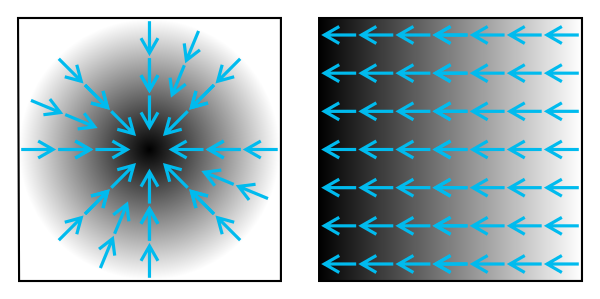
\includegraphics[height=3cm]{imageGradient}
	\caption{دو مثال از جهت‌گیری بردار‌های گرادیان در تصاویر}
	\label{gradImgEx}
\end{figure}
\subsection{در‌هم‌ریزی پوآسون}
در این قسمت، در‌هم‌ریزی پوآسون را به عنوان روشی برای ترکیب دو تصویر متفاوت در فضای گرادیان آورده‌ایم. تعریف مسئله و متغیر‌های مشخص‌شده در این قسمت از \cite{PoissonImageEditing} آورده شده‌است. ابتدا در شکل \ref{poissonSolve} متغیر‌ها را نمایش می‌دهیم و سپس به تعریف این متغیرها می‌پردازیم.
\begin{figure}[h!]
	\centering
	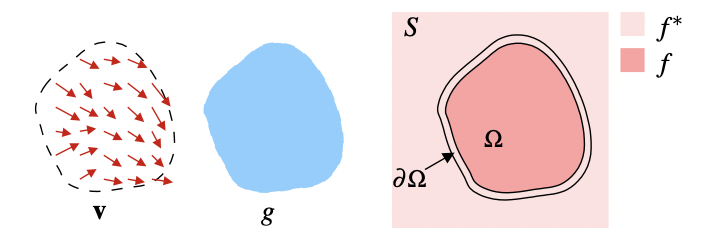
\includegraphics[height=3cm]{poissonSolve}
	\caption{نمایش متغیر‌های مورد استفاده در روش درهم‌ریزی پوآسون (از \cite{PoissonImageEditing})}
	\label{poissonSolve}
\end{figure}
در شکل \ref{poissonSolve}، متغیرها به این صورت تعریف می‌شوند:
\begin{itemize}
	\item 
	$g$ : تابع منبع
	\item 
	S : فضای مقصد
	\item 
	$\Omega$ : زیرمجموعه‌ای از فضای مقصد
	\item 
	$f$ : تابع درون‌یابی
	\item
	$f^*$ : تابع مقصد
	\item 
	\textbf{v} : میدان برداری (می‌تواند گرادیان g .باشد)
\end{itemize}
در مسئله‌ی درهم‌ریزی پوآسون، ما $f$ را طوری به دست می‌آوریم که بتواند هم مشخصات \lr{v} و هم مشخصات $f^*$ را حفظ کند. به این منظور یک مسئله‌ی بهینه‌سازی مطابق معادله‌ی \ref{variationalEq} تعریف می‌شود.
\begin{equation} \label{variationalEq}
	\min_f \iint_\Omega |\nabla f - \text{\textbf{v}} |^2 \quad \textrm{with} \quad f|_{\partial \Omega} = f^*|_{\partial \Omega} 
\end{equation}
به طوری که 
$\nabla f = \begin{bmatrix} \frac{\partial f}{\partial x} &  \frac{\partial f}{\partial y}\end{bmatrix}$ 
و 
$\text{\textbf{v}} = (u,v) = \nabla g$.

پاسخ معادله‌ی \ref{variationalEq} با پاسخ معادله‌ی زیر برابر خواهد بود:
\begin{equation} \label{poissonEq}
	\Delta f = \textrm{div}\ \text{\textbf{v}}\ \textrm{over}\ \Omega \quad \textrm{with} \quad f|_{\partial \Omega} = f^*|_{\partial \Omega} 
\end{equation}
به طوری که 
$\Delta f = \begin{bmatrix}\frac{\partial^2 f}{\partial x^2} + \frac{\partial^2 f}{\partial y^2}\end{bmatrix}$.
از طرف دیگر، داریم:
\begin{equation}
	\textrm{div}\ \text{\textbf{v}} = \frac{\partial u}{\partial x} + \frac{\partial v}{\partial y} = \frac{\partial^2 g}{\partial x^2} + \frac{\partial^2 g}{\partial y^2} = \Delta g
\end{equation}
که نشان می‌دهد با استفاده از این معادله‌ در حال یکسان‌سازی لاپلاس توابع \lr{$g$} و \lr{$f$} هستیم. این معادله، یک معادله پوآسون به همراه \gls{Dirichlet boundary conditions} است.
\newline
معادله‌ی \ref{poissonEq} پایه‌ی اصلی ویرایش تصاویر رنگی به روش پوآسون است. برای اجرای این روش در فضای رنگی، سه دفعه این معادله در سه کانال فضای رنگی انتخاب‌شده (لزومی بر \lr{RGB} بودن نیست)، به صورت مجزا اجرا می‌شود تا تصویر نهایی به دست آید.
\newline
با توجه به این موضوع که معادله‌ی \ref{poissonEq} را می‌توان به صورت مجزا برای هر پیکسل اجرا کرد، برای هر پیکسل مانند \lr{p}، می‌توان نوشت:
\begin{equation}
	\Delta f_p = \Delta g_p
\end{equation}
که با توجه به فیلتر پیچشی معرفی‌شده در بخش قبلی برای محاسبه‌ی لاپلاس در تصاویر، این معادله برای تصاویر به شکل زیر نوشته می‌شود:
\begin{equation}
	4f_p - \sum_{q \in N_p} f_q = 4g_p - \sum_{q \in N_p}  g_q
\end{equation}
که $N_p$ مجموعه‌ی همسایگی‌های پیکسل \lr{p} را نمایش می‌دهد. این معادله را می‌توان به صورت زیر نوشت:
\setcounter{MaxMatrixCols}{20}
\begin{equation} \label{linearPoisson}
	\begin{bsmallmatrix}0 & \ldots & 0 & -1 & 0 &  \ldots & -1 & 4 & -1 & 0 & \ldots & -1 & 0 & \ldots& 0\end{bsmallmatrix} 
	\begin{bsmallmatrix}f_1 \\ \vdots \\ f_{q1} \\ \vdots\\ f_{q2} \\ f_p \\ f_{q3} \\ \vdots \\ f_{q4} \\ \vdots \\ f_N \end{bsmallmatrix} = 
	\begin{bsmallmatrix}\Delta g_1 \\ \vdots \\ \Delta g_{q1} \\ \vdots\\ \Delta g_{q2} \\ \Delta g_p \\ \Delta g_{q3} \\ \vdots \\ \Delta g_{q4} \\ \vdots \\ \Delta g_N\end{bsmallmatrix}
\end{equation}
معادله‌ی \ref{linearPoisson} یک معادله خطی به شکل \lr{$Af = b$} است که به ازای هر پیکسل، یک سطر از ضرایب به بخش $A$ اضافه می‌شود. می‌توان این معادله را برای رسیدن به $f$، که تابع هدف ما و همان تابع درون‌یابی است، با روش‌های مختلف حل سیستم معادله‌های خطی به‌دست آورد. مشخص است ماتریس نهایی $A$، یک ماتریس $N*N$ خواهد بود. می‌توان نمایش داد این ماتریس همان ماتریس 
\lr{$(\nabla f)^T \nabla f$} 
و در نتیجه متقارن و \gls{Positive-Definite} است.
\subsection{واپیچش تصویر}
واپیچش در تصاویر زمانی اتفاق می‌افتد که خطوط صاف در تصویر، بعد از عکس‌برداری با دوربین، از صاف بودن خارج می‌شوند. واپیچش نوعی ابیراهی نوری است که اگرچه می‌تواند نامنظم باشد یا از الگوهای مختلف پیروی‌کند، اما اغلب به علت تقارن لنز تصویربرداری به طور شعاعی متقارن یا تقریبا متقارن است. این واپیچش‌های شعاعی معمولاً می توانند به عنوان واپیچش بشکه‌ای یا واپیچش بالشتکی طبقه‌بندی شوند، که در ادامه تعریف‌های این دو نوع واپیچش را آورده‌ایم. در شکل \ref{distortions} نیز می‌توان مثالی برای این دو واپیچش مشاهده کرد.
\begin{description}
	\item[واپیچش بشکه‌ای:]
در واپیچش بشکه‌ای، بزرگنمایی تصویر با فاصله‌گرفتن از مرکز تصویر کاهش می‌یابد. نتیجه‌ی ظاهری آن مانند تصویری است که به دور یک بشکه ترسیم شده‌است. لنزهای \gls{Fish-Eye} که نماهای نیمکره‌ای دارند، از این نوع واپیچش به عنوان راهی برای نمایش زوایای بیشتری از صحنه در تصویر محدود استفاده می‌کنند. در یک لنز برزگ‌نمایی، واپیچش بشکه‌ای در وسط تصویر ظاهر می‌شود و هر چه به کناره‌های تصویر نزدیک می‌شویم، این واپیچش بدتر خواهد‌شد.
	\item[واپیچش بالشتکی:]
در واپیچش بالشتکی، بزرگنمایی تصویر با فاصله‌گرفتن از مرکز تصویر افزایش می‌یابد. نتیجه‌ی قابل مشاهده این است که خطوطی که از مرکز تصویر عبور نمی‌کنند، به سمت داخل، یعنی مرکز تصویر، مانند یک بالشتک، خم می‌شوند.
\end{description}
\begin{figure}[h]
	\centering
	\subfloat[تصویر اصلی]{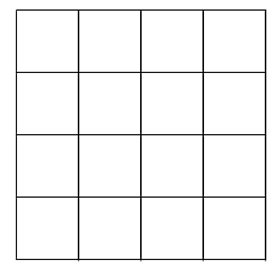
\includegraphics[height=4cm]{distortions-1}\label{distortions:f1}}
	\qquad
	\subfloat[واپیچش بالشتکی]{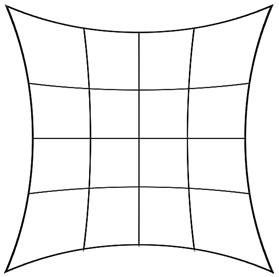
\includegraphics[height=4cm]{distortions-2}\label{distortions:f2}}
	\qquad
	\subfloat[واپیچش بشکه‌ای]{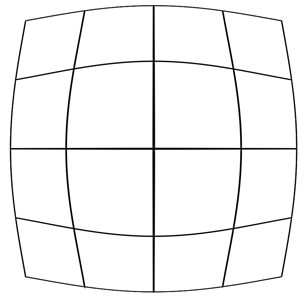
\includegraphics[height=4cm]{distortions-3}\label{distortions:f3}}
	\caption{دو نوع اصلی واپیچش در تصاویر}
	\label{distortions}
\end{figure}
\section{مروری بر مطالعات انجام‌شده}
در این قسمت تعدادی از پژوهش‌های مرتبط با هدف ما آورده شده‌است. این پژوهش‌ها در دو زمینه‌ی تولید بافت از یک تصویر و اتصال تصاویر برای تولید سراسرنما صورت گرفته‌اند. برای بررسی جامع پژوهش‌های انجام‌شده در زمینه‌ی تولید بافت از یک تصویر به \cite{jetchev2017texture} و \cite{survey2020} مراجعه کنید. این قسمت با استفاده از \cite{szeliski2011computer} نوشته شده است که سعی کردیم در طول مسیر پژوهش از این کتاب به عنوان مرجع اصلی استفاده کنیم.
\subsection{تولید بافت از یک تصویر} \label{texSynLit}
مسئله‌ی تولید بافت را می توان به صورت تولید بافت با استفاده از ورودی یک نمونه‌ی کوچک از آن، توصیف کرد. رویکردهای سنتی برای تولید بافت تلاش می‌کنند خروجی‌های تولید‌شده با طیف تصویر منبع مطابقت داشته باشند و در عین حال \gls{Structured Noise} ایجاد کنند. الگوریتم‌های تولید بافت از یک تصویر به‌طور متوالی پیکسل‌های بافت را برای جست‌وجوی همسایگی‌هایی در بافت منبع که مشابه تصویر فعلی تولید شده هستند، استفاده می‌کنند\cite{nonParam}. در اجرا، مشابه‌ترین همسایگی را در نمونه‌ی بافت پیدا می‌کنند و سپس تمام همسایه‌های دیگر را در فاصله
\lr{$d=(1+\epsilon)$} 
  با
\lr{$\epsilon=0.1$}  
  درنظر می‌گیرند. آنها همچنین پیکسل‌های مناسب برای ادامه‌ی تولید بافت را به صورت تصادفی و با وزن انتخاب‌شده با معیار فاصله‌ی d برای پیکسل‌های همسایگی مناسب، انتخاب می‌کنند.

برای تسریع این فرآیند و بهبود کیفیت ظاهری آن، \cite{treeVecQuant} این روش را با استفاده از فرآیند تولید \gls{Coarse-to-Fine} گسترش دادند، جایی که سطوح درشت‌تر هرم، که قبلاً تولید شده‌اند، نیز در طول یافتن پیکسل مناسب در نظر گرفته می‌شوند\cite{deBonet}. برای تسریع یافتن نزدیکترین همسایه، از \gls{Quantization} برداری با ساختار درختی استفاده می‌شود. یک نسخه بسیار سریع‌تر در جستجوی مشابه‌ترین پیکسل همسایه، الگوریتم به‌روزرسانی تکراری تصادفی \gls{Patch-Based} است که توسط \cite{patchMatch} توسعه داده شده است. محققین در
\cite{imageQuilting} 
روشی برای افزایش سرعت و بهبود ویژگی‌های ظاهری تصویر تولید‌شده‌ی نهایی پیشنهاد کردند. به جای تولید یک پیکسل در هر زمان، بلوک های مربعی که با یکدیگر هم‌پوشانی دارند برای استفاده در جست‌وجوی مشابه‌ترین بلوک با بافت تولید‌شده‌ تا به آن زمان استفاده می‌شوند. هنگامی که بلوک‌های مناسب انتخاب شدند، \gls{Seam} بین بلوک‌های همپوشانی جدید با استفاده از برنامه‌نویسی پویا تعیین می‌شود. از آنجا که این فرآیند شامل انتخاب تکه‌های کوچک و اتصال آن‌ها به یکدیگر است، آن‌ها سیستم خود را \gls{Image Quilting} می‌نامند.

ادامه‌ی پژوهش‌های انجام شده در این زمینه، به صورت خاص‌منظوره نسبت به هدف استفاده از بافت انجام شده‌اند. به طور مثال در زمینه‌ی پرکردن شکاف در تصویر، \cite{criminisiPerezInpaint} روشی را با استفاده از تولید بافت مبتنی بر نمونه ارائه می‌دهد که در آن، ترتیب ترکیب با مقادیر گرادیان در امتداد مرز منطقه تعیین می‌شود. \cite{wexlerIrani} نیز از روشی مشابه برای پر کردن شکاف در ویدئو‌ها استفاده می‌کند. در جدیدترین پژوهش‌ها تلاش‌شده با استفاده از یادگیری عمیق، روش‌هایی برای بهبود ویژگی‌های ظاهری تصویر تولید‌شده‌ی نهایی ارائه شود\cite{nazeri2019edgeconnect}\cite{yi2020contextual}. در تعدادی از این پژوهش‌ها، استخراج ساختار و گسترش بافت به ابعاد دلخواه، همگی توسط یک شبکه‌ عصبی با استفاده از لایه‌های پیچشی انجام شود\cite{gatys2015texture}\cite{risser2020optimal}.
\subsection{ترکیب تصاویر در فضای گرادیان}
بازسازی تصاویر از فضای گرادیان آن‌ها، از زمینه‌های قدیمی در بینایی ماشین است\cite{HornRV} که اولین استفاده‌ها از این روش در ثبات روشنایی\cite{Horn1974DeterminingLF}، شکل از سایه‌زنی\cite{shapeFromShading} و استریو فوتومتریک\cite{Woodham1994GradientAC} بوده است. ایده‌های مشابهی برای بازسازی تصاویر با استفاده از لبه‌های موجود در تصویر\cite{elderGoldberg}، از بین بردن سایه در تصاویر\cite{weissShadow} و جداسازی بازتاب نور از تصویر\cite{levinReflect1}\cite{levinReflect2} نیز استفاده شده است.

\cite{PoissonImageEditing}
 نشان می‌دهد چگونه می‌توان از بازسازی در فضای گرادیان برای ترکیب یک تصویر در تصویر دیگر استفاده کرد. به جای تکرار کردن مستقیم پیکسل‌ها، از تکرار مقادیر گرادیان تصاویر استفاده می‌شود. پیکسل‌ها در انتها با استفاده از حل کردن یک معادله‌ی پوآسون برای یکسان‌سازی محلی مقادیر گرادیان با توجه به شرایط مرزی دیریکله در ناحیه هم‌پوشانی محاسبه می‌شوند. در پژوهش‌های قدیمی‌تر، \cite{Peleg1981EliminationOS} یک تابع هموارساز معرفی می‌کند تا برای اطمینان از پایداری تصویر در ناحیه هم‌پوشانی از آن استفاده شود.

\cite{agarwala2004}
 این ایده را برای استفاده در مسئله‌ی ترکیب چند تصویر ورودی بسط داده است که دیگر صحبت از مقصد برای هموارسازی در ناحیه هم‌پوشانی معنا ندارد. در عوض، از گرادیان هر منبع در معادله‌ی پوآسون استفاده می‌شود و این معادله با توجه به \gls{Neumann boundary conditions} حل می‌شود. به جای حل مستقیم معادله پو‌آسون، در این روش از حداقل‌سازی یک مسئله‌ی متغیر استفاده می‌شود که در معادله‌ی \ref{agarwala} آمده است.
\begin{equation} \label{agarwala}
	\min_{C(x)} ||\nabla C(x) - \nabla \tilde{I}_{l(x)}(x)||^2
\end{equation} 
فرم گسسته‌ی این معادله را می‌توان با استفاده از تعدادی معادله‌ی قیود گرادیان به صورت زیر نوشت:
\begin{gather}
	C(x+\hat{i}) - C(x) = \tilde{I}_{l(x)}(x+\hat{i}) - \tilde{I}_{l(x)}(x) \qquad \textrm{and}\\
	C(x+\hat{j}) - C(x) = \tilde{I}_{l(x)}(x+\hat{j}) - \tilde{I}_{l(x)}(x) \qquad \quad
\end{gather}
که 
\lr{$\hat{i} = (1,0)$} 
و 
\lr{$\hat{j} = (0,1)$} 
بردارهای یکّه در جهت محور‌های $x$ و $y$ هستند. آن‌ها سپس این مسئله‌ی حداقل مربعات پراکنده را حل می‌کنند. از آنجایی که این سیستم معادلات فقط تا یک حد افزایشی تعریف شده است، در پژوهش از کاربر خواسته می‌شود مقدار یک پیکسل را مشخص کند. در عمل، انتخاب بهتر ممکن است جهت‌دهی جزءی راه‌حل به سمت بازتولید مقادیر رنگ اصلی تصویر نهایی باشد.

به منظور تسریع حل این سیستم خطی پراکنده، محققان در \cite{fattal} از \gls{Multigrid} استفاده می کنند، در حالی که پژوهش شرح داده‌شده از روش گرادیان استفاده می کند\cite{56188}\cite{10.1145/1141911.1142005}\cite{10.1145/2070781.2024211}\cite{10.1145/2461912.2461992}. پژوهش بعدی، \cite{10.1145/1275808.1276495} نشان می‌دهد که چگونه استفاده از یک نمایش \gls{Quadtree} برای راه‌حل می‌تواند محاسبات را با کاهش حداقلی دقت، تسریع کند. \cite{fastPoisson} بیان می‌کند ترکیب در فضای لگاریتمی، یا استفاده از جمع به جای ضرب، ترجیح داده می‌شود، زیرا مطابقت تصویر نهایی تولید‌شده با تفاوت‌های نوری بافت در ناحیه هم‌پوشانی بیشتر است. نتایج ترکیب تصاویر به‌دست‌آمده مطلوب است، اگرچه هنگام کپی کردن مقادیر گرادیان بزرگ در نزدیکی ناحیه هم‌پوشانی باید دقت شود تا \gls{Double Edge} ایجاد نشود.

کپی کردن گرادیان‌ها به طور مستقیم از تصاویر منبع پس از قرار دادن ناحیه هم‌پوشانی، تنها یک رویکرد برای ترکیب تصاویر در فضای گرادیان است. \cite{SeamlessStitching} چندین نوع مختلف از این رویکردها را بررسی می‌کند که آنها را 
\lr{Gradient-domain Image Stitching}
یا \lr{GIST} می‌نامند. تکنیک‌هایی که آنها بررسی می کنند، شامل \gls{Feathering} گرادیان‌ها از تصاویر منبع، و همچنین استفاده از \gls{L1-Norm} در انجام بازسازی تصاویر از فضای گرادیان، به جای استفاده از \gls{L2-Norm} مانند معادله \ref{agarwala} است. روش پیشنهادی آن‌ها بهینه سازی نُرم یک تابع هزینه‌ی پوشش‌گذاری بر روی گرادیان‌های تصویر اصلی (که \lr{GIST1-l1} می نامند) است. از آنجایی که بهینه‌سازی نُرم یک با استفاده از برنامه‌نویسی خطی می تواند کند باشد، آنها الگوریتم سریع‌تری را در یک چارچوب چندشبکه‌ای توسعه می‌دهند. مقایسه‌ی بصری بین رویکرد ترجیحی آنها و \cite{agarwala2004} نتایج مشابهی را نشان می‌دهد، در حالی که به طور قابل توجهی از الگوریتم‌های ترکیب هرمی و پوشش‌گذاری بهتر است.